\chapter{Architecture}
\label{chapter:dynamic resource}
This section illustrates and describes the high level architecture of the software implemented along with a few protocol sequence diagrams. It will help to understand at a high level about the components which form a part of this system to support the new approach of invasive computing and how will its components interact with each other through new protocols or extensions of existing protocols in order to integrate such an invasive resource management into existing batch systems.\\ \\
%%%%%%%
The following page shows the software architecture of how invasive resource management can be supported with a traditional resource manager and how exactly the new software components will fit into the existing software hierarchy. The \ref{fig:7} relates closely to how SLURM is organized since the intention of this work would be to demonstrate the support for invasive computing with the help of SLURM as a resource manager.
\begin{itemize}
\item The top layer is that of the core resource management component which has access to job queues. In this architecture, it will now have access to not only the queue for the legacy(static) jobs but also invasive job queue(jobs submittted to invasic partition that supports invasive computing).
\item In a traditional setup the top layer will perform the task of job scheduling as well. This means that it will select a job(s) from the queue of jobs based on the current state of resources and many other factors to dispatch it to the traditional process manager below in the hierarchy. The process manager then takes the responsibility of launching these jobs on the allocated resources in the partition and managing them for their full lifetime. In case of parallel jobs, it will manage the job in a parallel environment along with facilitating the communication amongst the parallel tasks/processes with the help of a PMI(Process Manager Interface). The process manager may also spawn slave daemons on each of the nodes which are a part of the resource allocation for a single job to manage them more effectively.
\begin{figure}[!htbp]
\centering
\includegraphics[width=1.0\textwidth, height=185mm]{./figures/"iRM Architecture".pdf}
%\includegraphics[width=1.0\textwidth, height=185mm]{./figures/"software architecture".eps}
\caption{Invasive Resource Management Architecture}
\label{fig:7}
\end{figure}
\item As discussed in the previous chapter, an independent invasive resource management component by the name "iRTSched" will be implemented which needs to communicate with the batch scheduler and influence the scheduling decisions taken by it. The iRTSched sits between the top layer and the process manager.
\item A new job scheduler specifically for invasive jobs needs to be integrated into the existing batch system. This is due to the reason that the scheduler for invasive jobs will work in a different manner based on the approach described earlier in comparison to the legacy job scheduler for static jobs. In case of SLURM which has a modular design with several optional plugins, a new plugin by name "iBSched" will be implemented for SLURM to handle job scheduling specifically for invasic jobs.
\item Communication between iRTSched and iBSched will involve the negotiation protocol as explained in the previous chapter but will also include periodic / event-driven feedbacks being sent by iRTSched to iBSched. These will contain some useful information about the current state of the running jobs, their energy consumption, other job characteristics etc. This communication will also additionally support a means to service urgent jobs immediately.
\end{itemize}
%\begin{figure}[!htbp]
%\centering
%\includegraphics[width=1.0\textwidth, height=185mm]{./figures/"iRM Architecture".pdf}
%\includegraphics[width=1.0\textwidth, height=185mm]{./figures/"software architecture".eps}
%\caption{Invasive Resource Management Architecture}
%\label{fig:7}
%\end{figure}
\textbf{Communication Phases}
\begin{itemize}
\item \textbf{\textit{Protocol Initialization:}} This phase basically establishes the initial environment between the communicating parties (iBSched and iRTSched) for proper communication later on. Successful initialization of this phase prepares both the parties to start negotiating based on the negotiation protocol described in the following points. During this protocol initialization various parameters such as protocl version, maximum attempts for negotiation, timer intervals and several others could be exchanged to set up the internal data structures and configuration tables for both the communicating parties. This protocol is a bi-directional communication.
\item \textbf{\textit{Protocol Finalization:}} This phases signals the end of the communication between iRTSched and iBSched using negotiation protocol. It leads to a safe termination of this communication followed by the release of any internal data structures allocated earlier along with configuration parameters. This results in consistent behaviour of both the communicating parties which can then proceed to safely terminate and exit. This protocol is a bi-directional communication.
\begin{figure}[h]
\centering
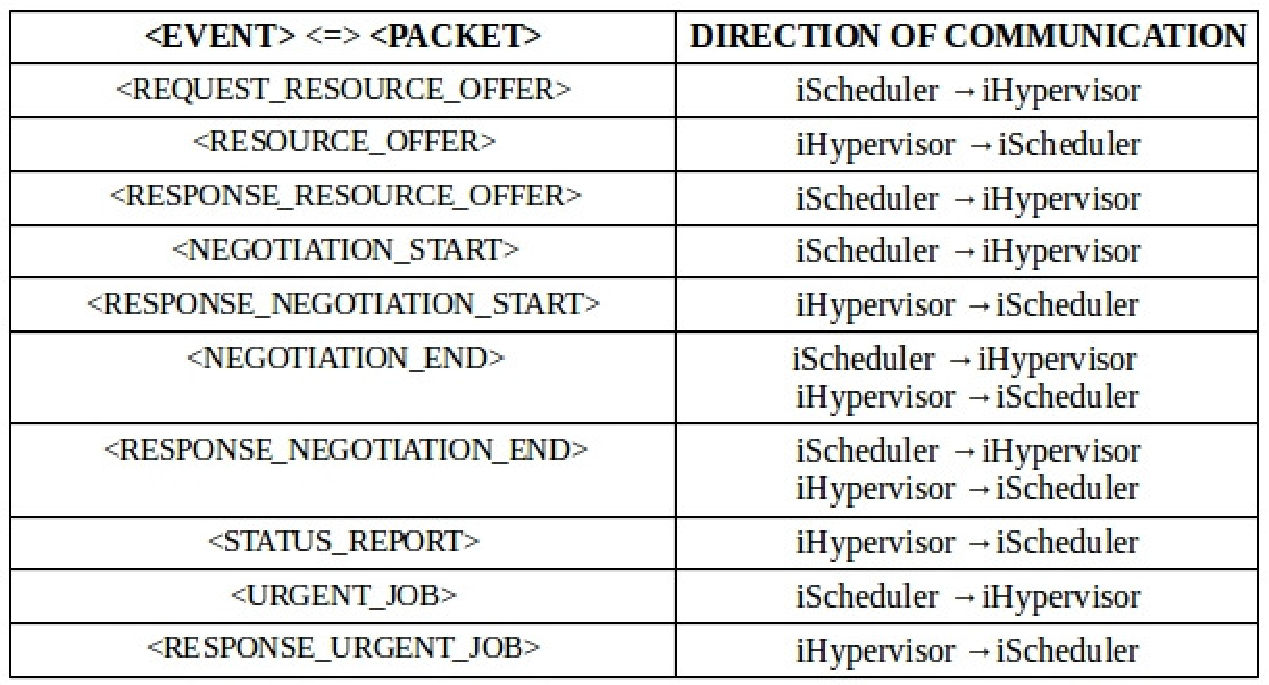
\includegraphics[width=1.0\textwidth, height=100mm]{./figures/table.pdf}
%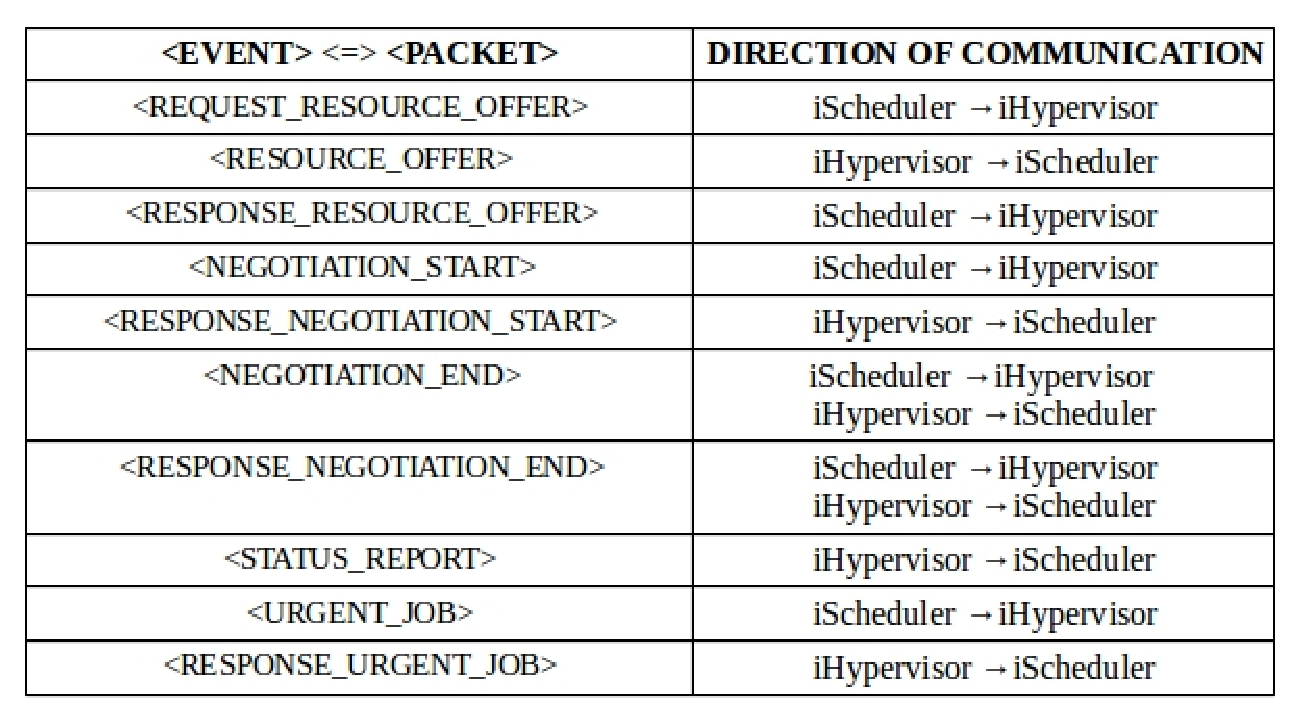
\includegraphics[width=1.0\textwidth, height=80mm]{./figures/table.eps}
\caption{Message Types}
\label{fig:8}
\end{figure}
\item \textbf{\textit{Negotiation:}} This is the most important phase in this whole approach to support invasive computing as discussed in the previous chapter. It is the phase during which both iRTSched and iBSched are negotiating with each other till they reach an agreement. If they do not then they continue till a certain limit to the number of negotiating attempts are reached after which both of them just agree in their final attempt closing the current negotiation. After this a new transaction of negotiation will begin at some later point of time.
\item \textbf{\textit{Feedback:}} This concerns the periodic / event-driven feedback sent by the iRTSched to the iBSched containing useful information as mentioned earlier. iRTSched will also send a performance model of every completed job in the feedback that can be stored in some database as a part of the history of executions for this job. This will help the iBSched in the future if the same job is submitted when there will be additional performance specific information available about this job that can be used by the batch scheduling algorithm to make better decisions for this job. This protocol is a uni-directional communication.
\item \textbf{\textit{Urgent Jobs:}} This protocol concerns the support for urgent jobs. At any given point of time a cluster or supercomputing center may want to support very high priority jobs immediately without any further delay. By introducing support for invasive computing, it makes it all the more feasible to help run these urgent jobs immediately by either shrinking the resources of other jobs or suspending/Killing them.
\end{itemize}
%%%%%%%%%%%%%%%%%
\section{Dynamic Resource Management}
\textbf{\textit{Separation of Concerns: }}In this thesis, We explore the idea of separating the concerns of batch and runtime scheduling into
two different software layers / components in contrast to the existing systems where both are merged together. A negotiation protocol will be implemented as a means of communication between the two. The motivation behind the negotiation protocol is the conflicting set of objectives between batch scheduler(user perspective: faster response time, fairness for jobs etc.) and run time scheduler(system perspective: maximize utilization, throughput, energy efficiency etc.). The role of the batch scheduler is to forward jobs to a runtime scheduler which is managing the resources in the partition(s) and supports runtime scheduling of adaptive applications. Runtime scheduler will make intelligent expand / shrink decisions by observing scalability behavior of the running applications and use it to predict future resource requirements. The proposed protocol will also allow us to integrate such adaptive resource management systems into existing batch systems and thereby allowing for an easy migration from legacy system to invasive resource management systems. Negotiation also helps us to realize a dynamic and flexible scheduling strategy by balancing the conflicting objectives at the two layers.\\ \\
%%%%%%%%%%%%%%%
We will briefly look at the important components in this architecture that work together in order to support adaptive applications on HPC systems by dynamically managing the resouce allocation of running jobs. 
\subsection{Invasive Batch Scheduler}
The purpose of a batch scheduler is to select jobs from its queue according to some algorithm and dispatch this to the runtime scheduler. This is similar to a long term scheduler which by its definition: admits new processes to the system and controls the degree of multiprogramming( number of processes in memory). The batch scheduler for HPC workloads also does something similar but it is also merged with runtime scheduler. In this work, we have separated the two because of which it now looks analagous to long term scheduler(batch scheduler) that admits jobs into the system and a short term scheduler(runtime scheduler) which will manage the running / ready jobs using either space sharing or time sharing. Batch scheduler runs less frequently and there may be quite a lot of time gap when the next job may be admitted into the system. This depends upon available resources, any events like job termination, completion etc. 
\subsection{Invasive Run Time Scheduler}
\subsection{iMPI Process Manager}
\section{Negotiation Protocol}
\subsection{Protocol Sequence Diagrams}
%\vspace{-0.15in}
\begin{figure}[!htbp]
%\begin{figure}[H]
\centering
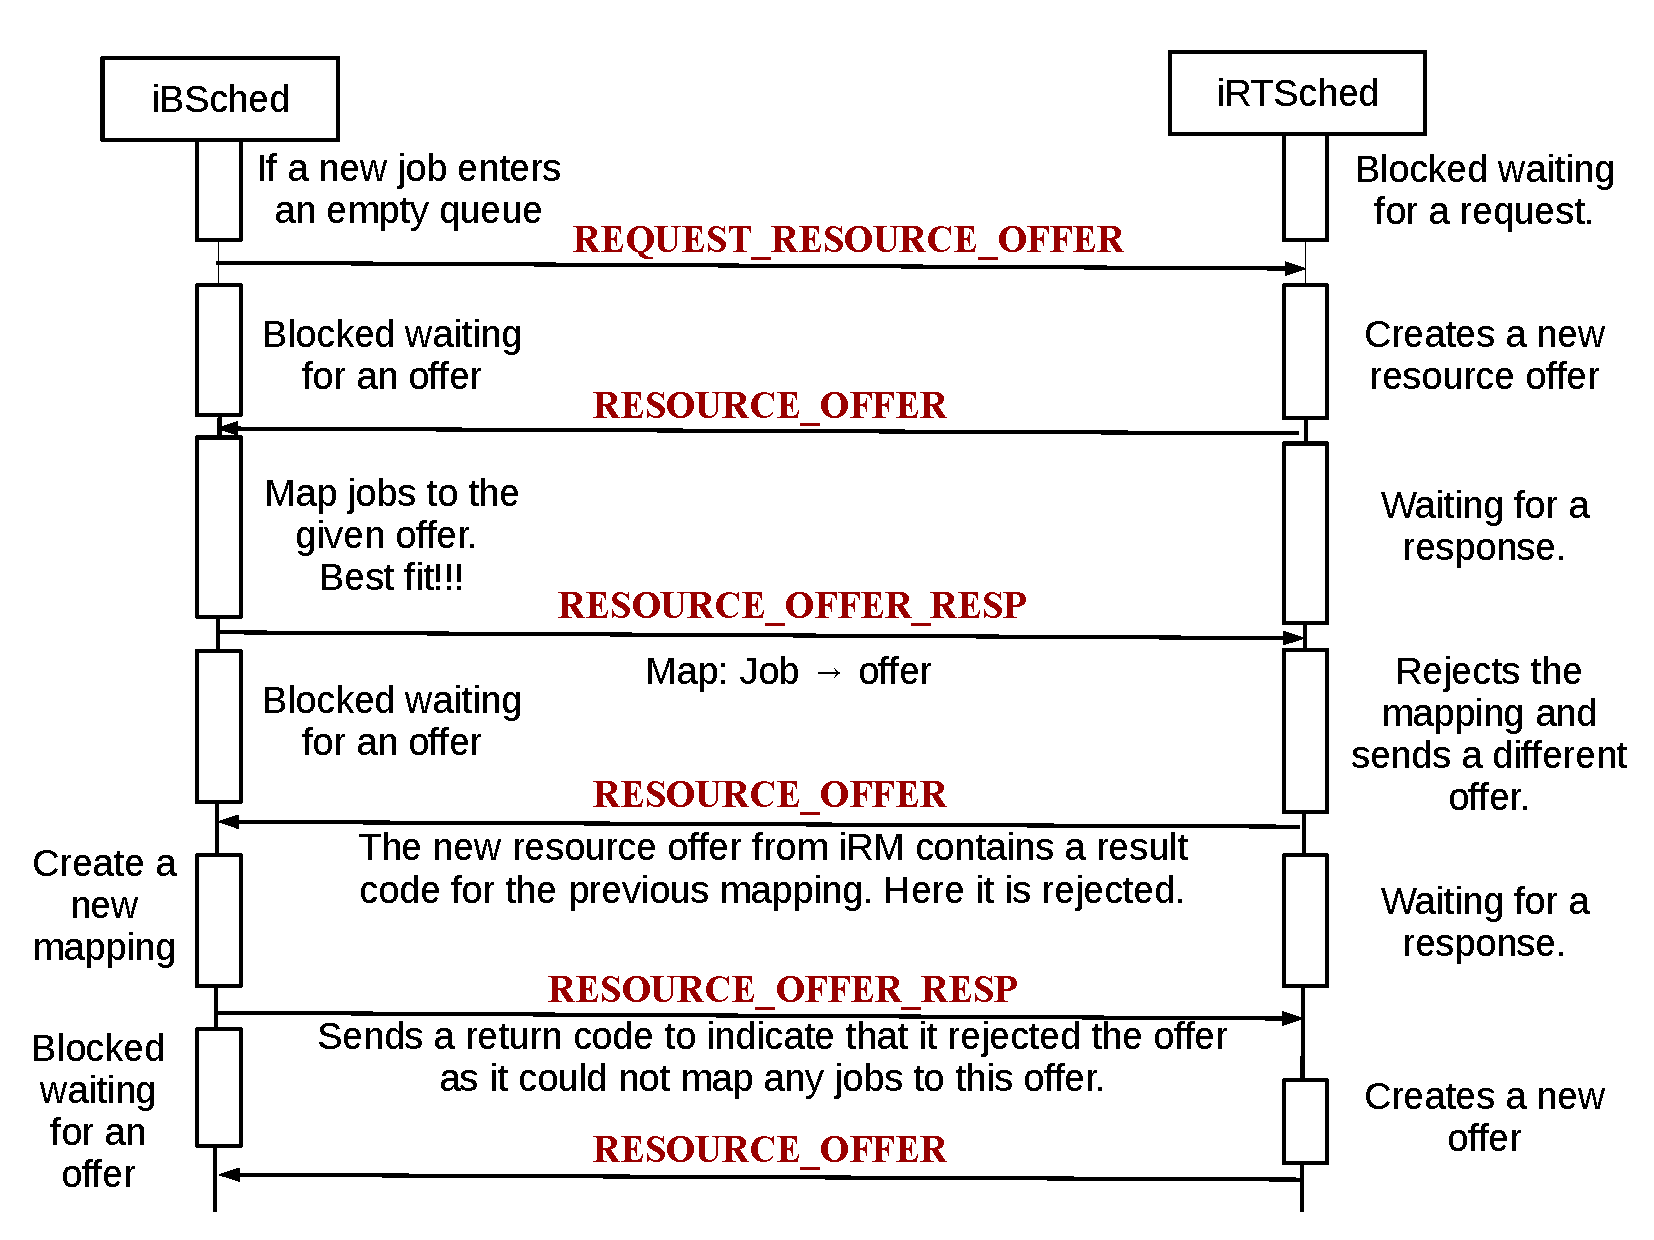
\includegraphics[width=1.0\textwidth, height=100mm]{./figures/scenario1.pdf}
%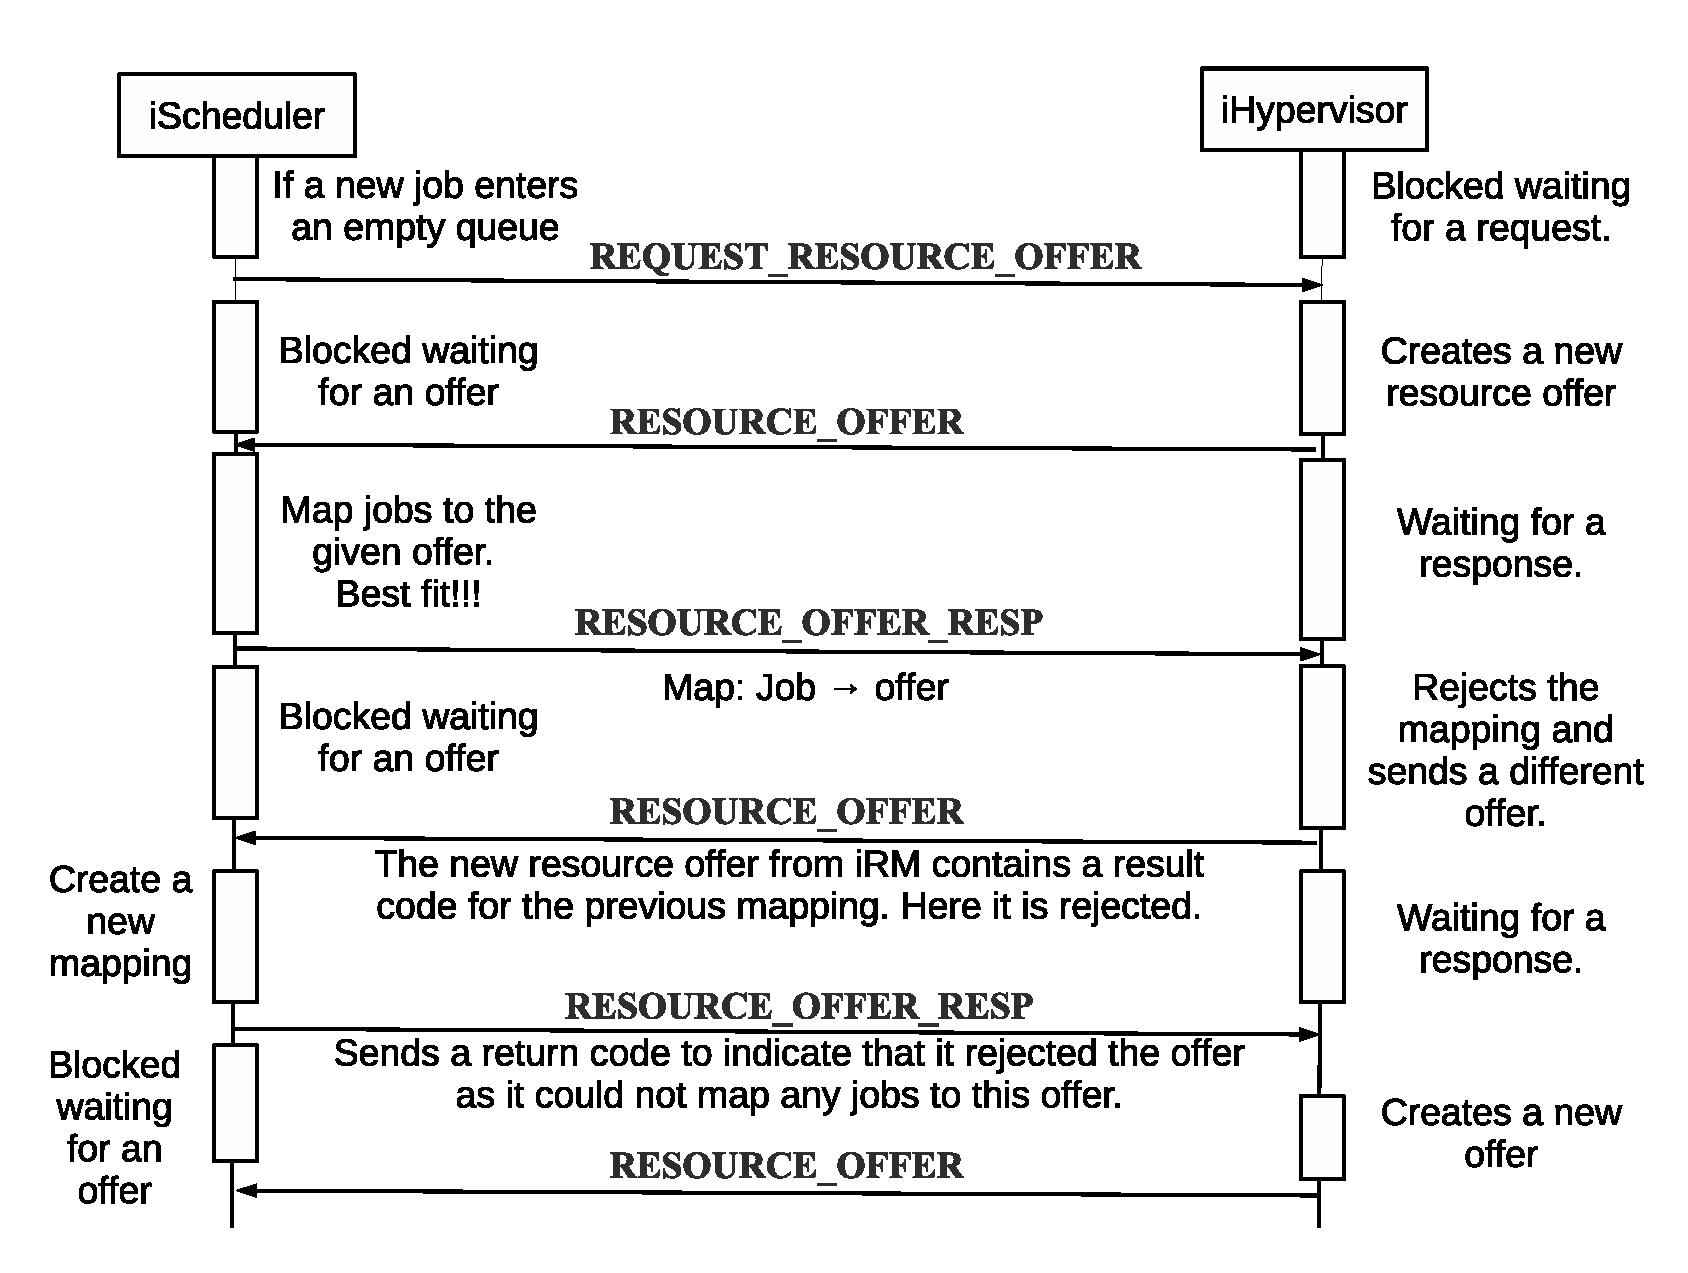
\includegraphics[width=1.0\textwidth, height=100mm]{./figures/figures.eps}
\caption{Scenario 1}
\label{fig:Seq1}
\end{figure}
\begin{itemize}
\item Above diagram illustrates a scenario where both iBSched and iHpervisor are negotiating with each other. The scenario is continued in the next page. \ref{fig:Seq2} illustrates another scenario where negotiations may stop when job queue becomes empty and iHypevisor then will wait for a request from iBSched for a resource offer that will happen when new jobs arrive.
\item iBSched makes scheduling decisions at a coarser level of granularity which is nodes whereas iRTSched does at the granularity of cores and sockets. Both will negotiate with each other till they reach an agreement.
\item It is an event based scheduling which means iBSched makes a scheduling decision only when it is triggered by receiving a resource offer from iRTSched. It is only at the start when there are no jobs in the queue and during the operations when the queue may become empty that the iBSched will have to explicitly send a request message to iRTSched for a resource offer otherwise at all other times scheduling is event based.
\end{itemize}
%\label{fig:Seq1}
%\end{figure}
\begin{figure}[!htbp]
\vspace{-0.25in}
\centering
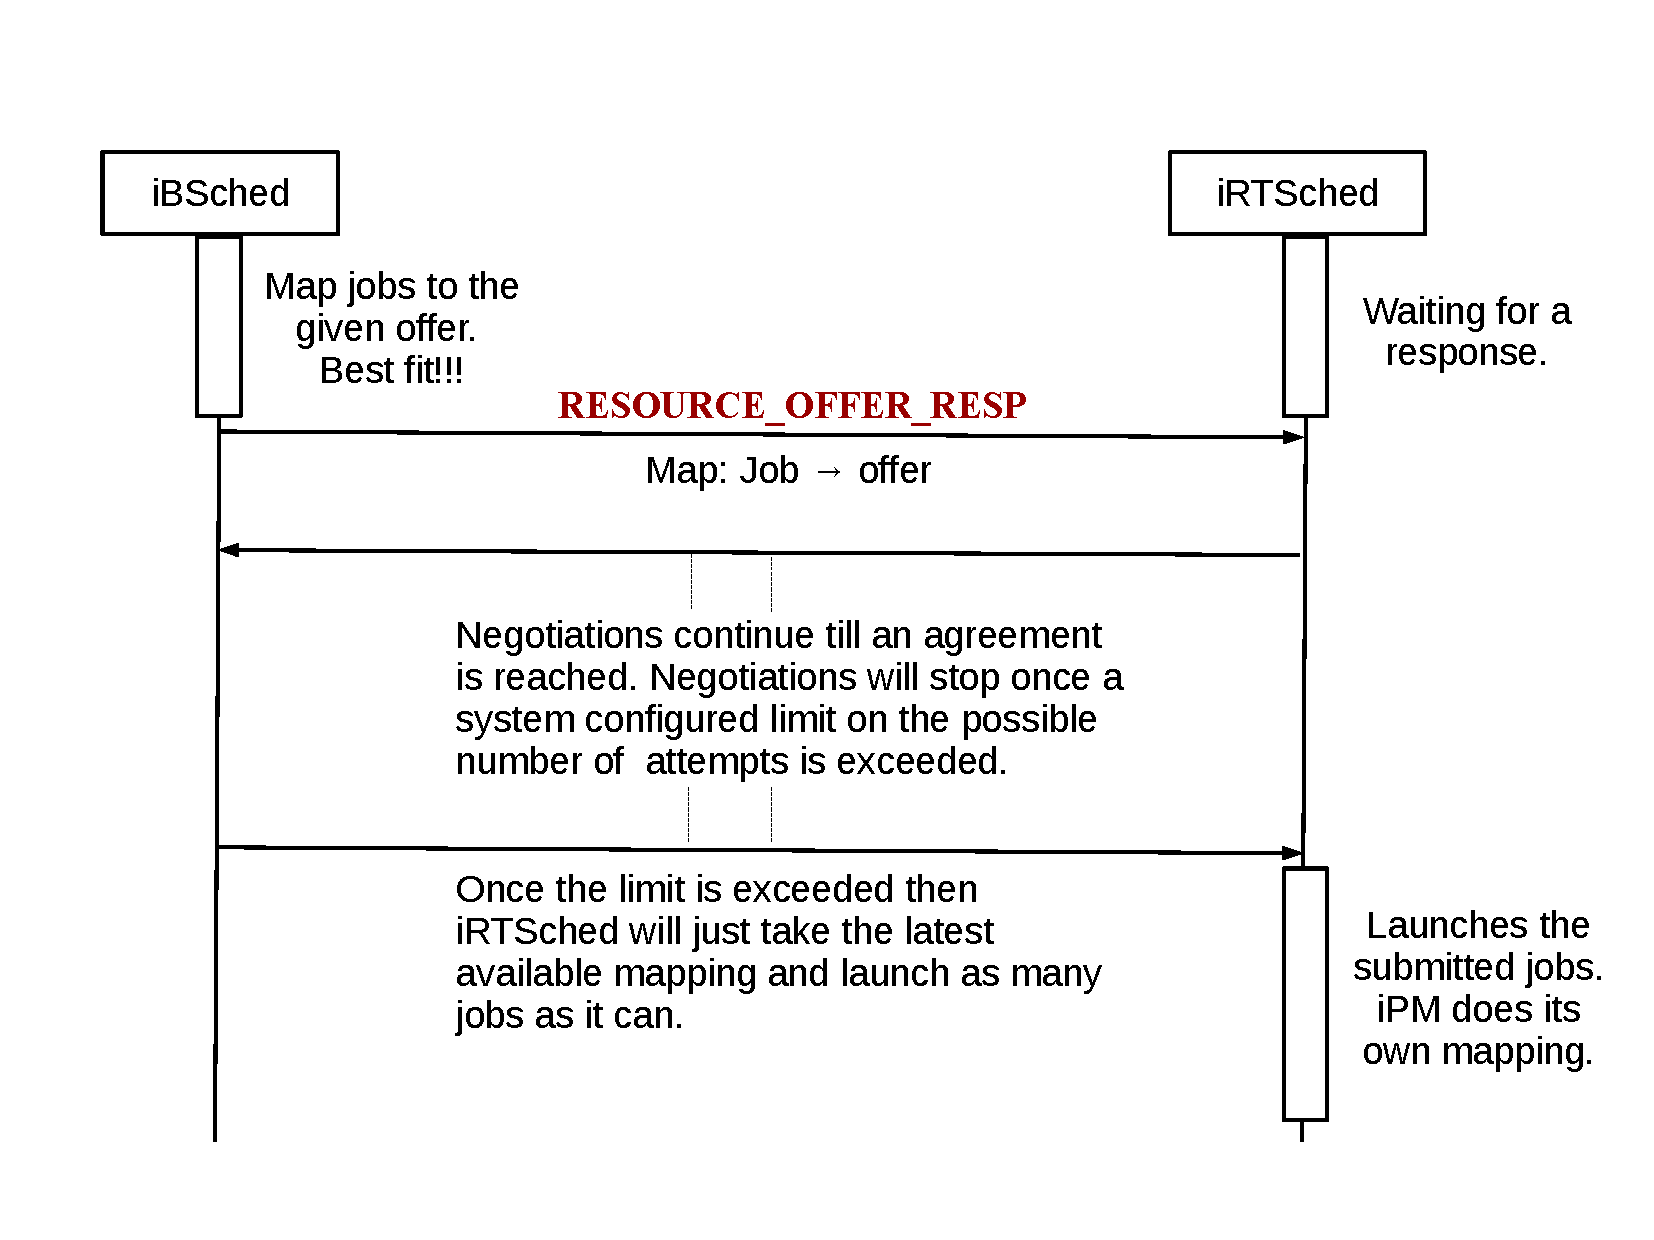
\includegraphics[width=0.9\textwidth, height=100mm]{./figures/scenario1contd.pdf}
%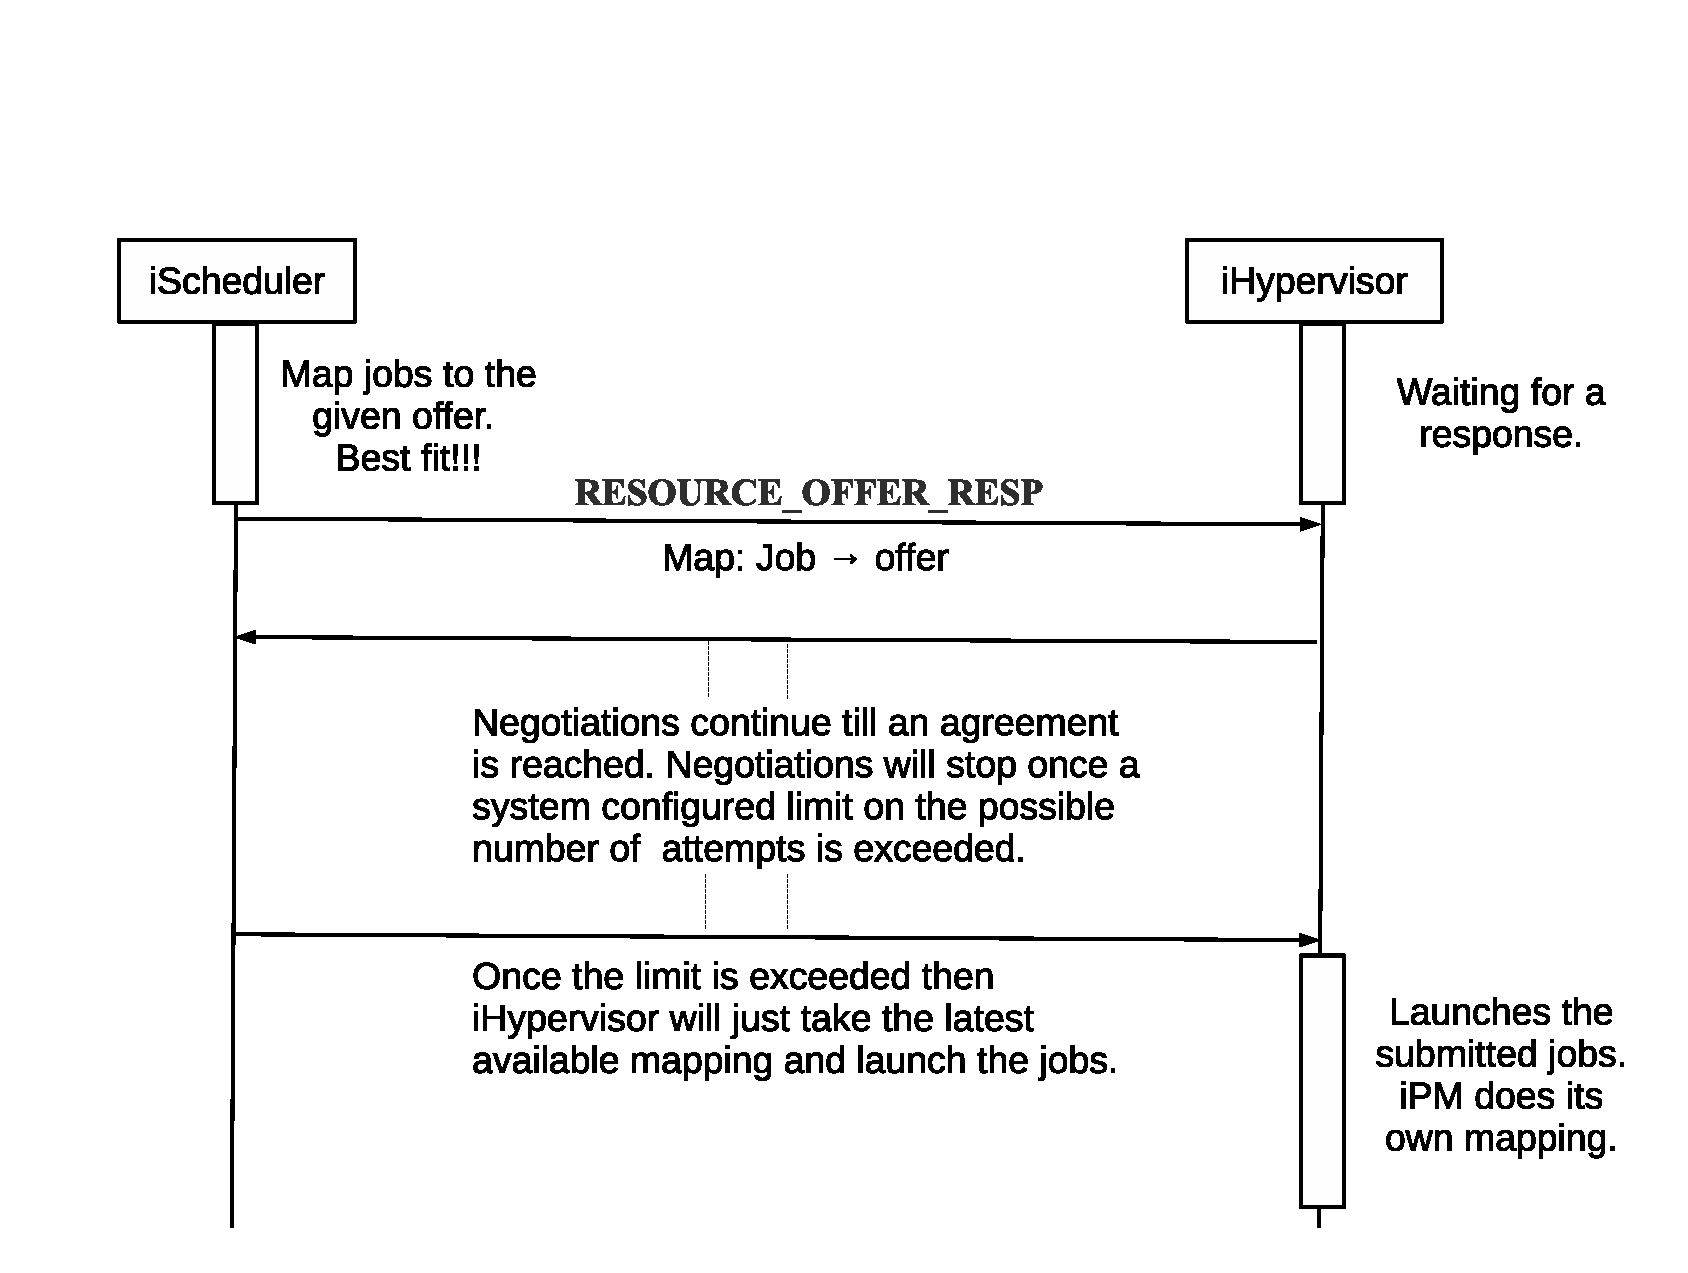
\includegraphics[width=0.9\textwidth, height=100mm]{./figures/figures1.eps}
\caption{Scenario 1 contd.}
\label{fig:Seq1}
%\vspace{-0.10in}
\end{figure}
\begin{figure}[!htbp]
%\vspace{-0.15in}
\centering
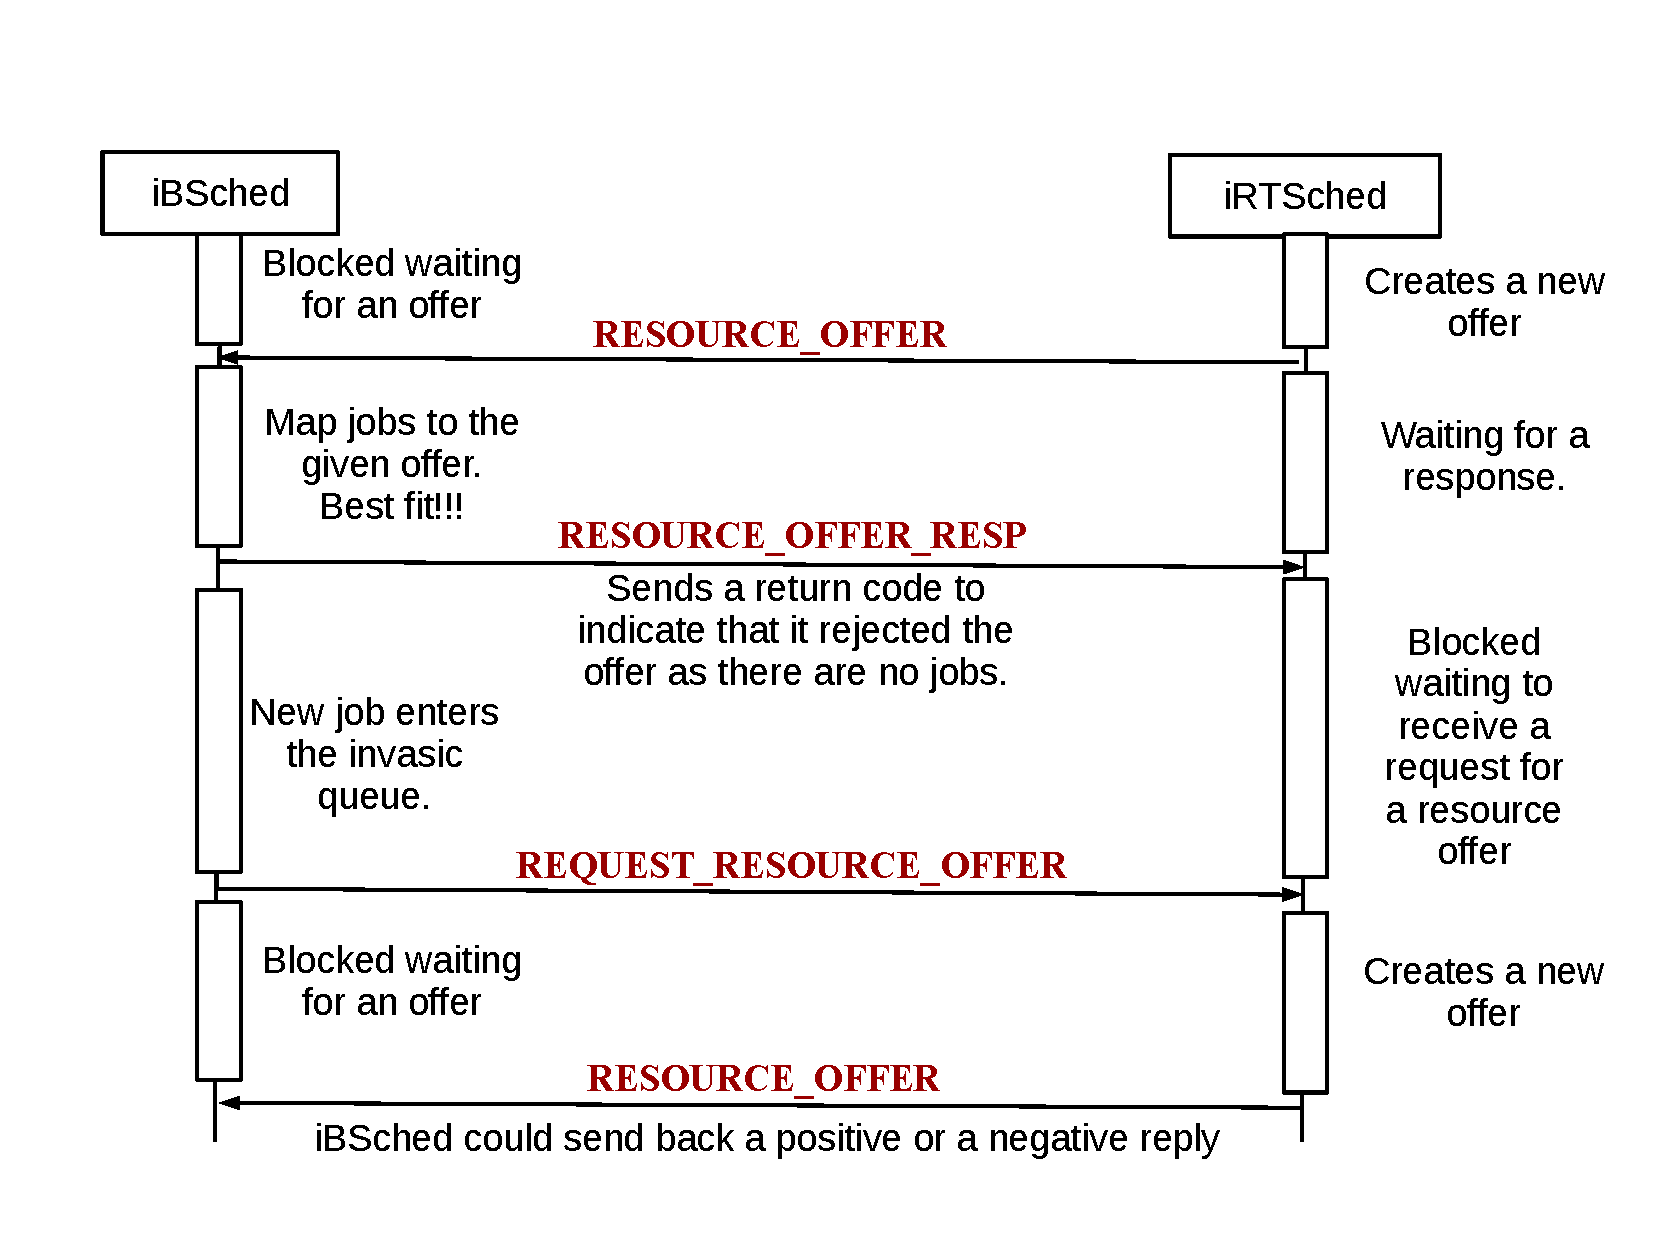
\includegraphics[width=0.9\textwidth, height=100mm]{./figures/scenario2.pdf}
%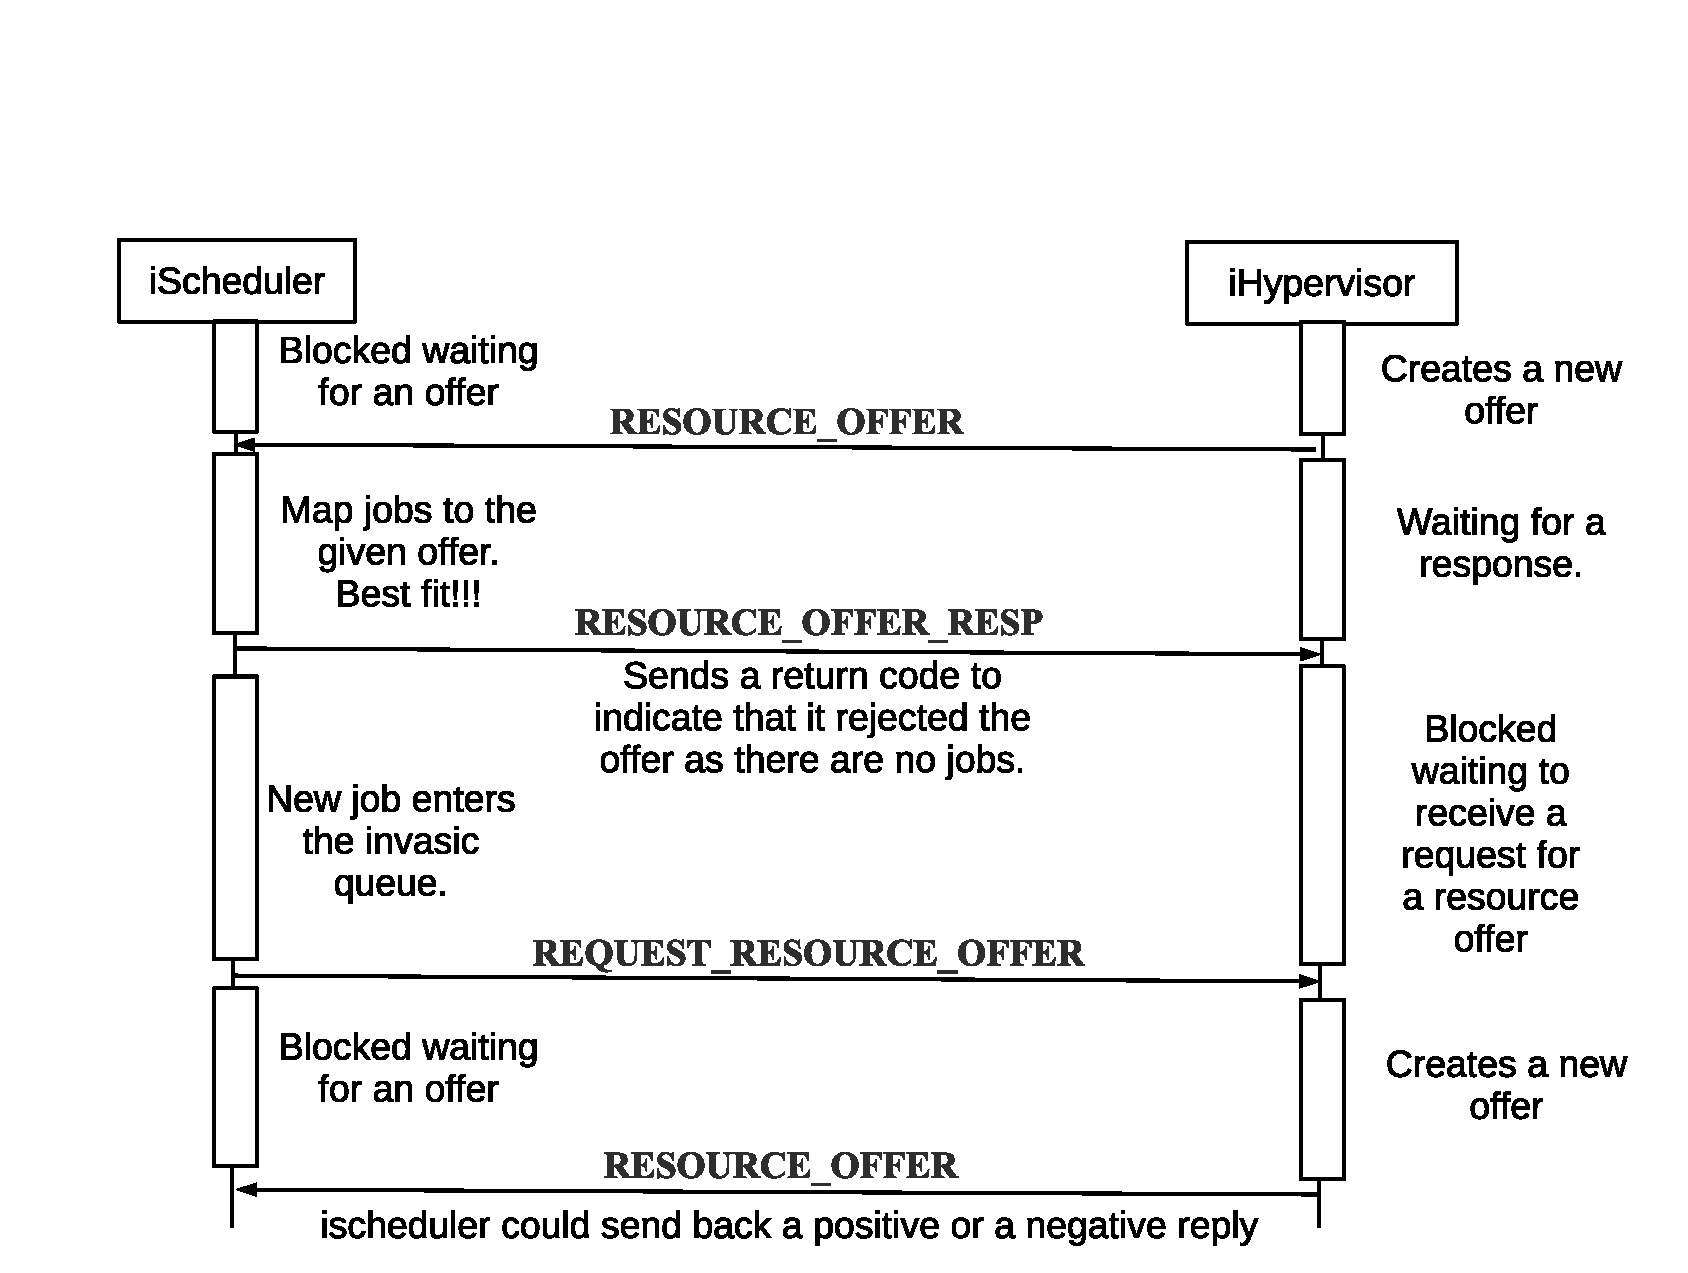
\includegraphics[width=0.9\textwidth, height=100mm]{./figures/figures2.eps}
\caption{Scenario 2}
\label{fig:Seq2}
\end{figure}
%\subsection{State Machine Diagrams}
This section focuses on iBSched and a thread iRM\_AGENT that it spawns which is the one responsible for all the communication with the iRTSched including spawning other agent threads for handling feedbacks and urgent jobs.
%\vspace{10mm}
\begin{figure}[h]
\centering
%\includegraphics[width=1.0\textwidth, height=150mm]{./figures/"iRM Agent".pdf}
\includegraphics[width=1.0\textwidth, height=150mm]{./figures/"iRM Agent".eps}
\caption{iRM Agent}
\label{fig:Init}
\end{figure}
\begin{itemize}
\item Above diagram and the ones in the following pages illustrate state machine diagrams for few of the communication phases described earlier starting first with a general diagram of how the mulithreaded component iRM agent inside iBSched starts up and shuts down.
\end{itemize}
\vspace{-20mm}
\begin{figure}[h]
\centering
%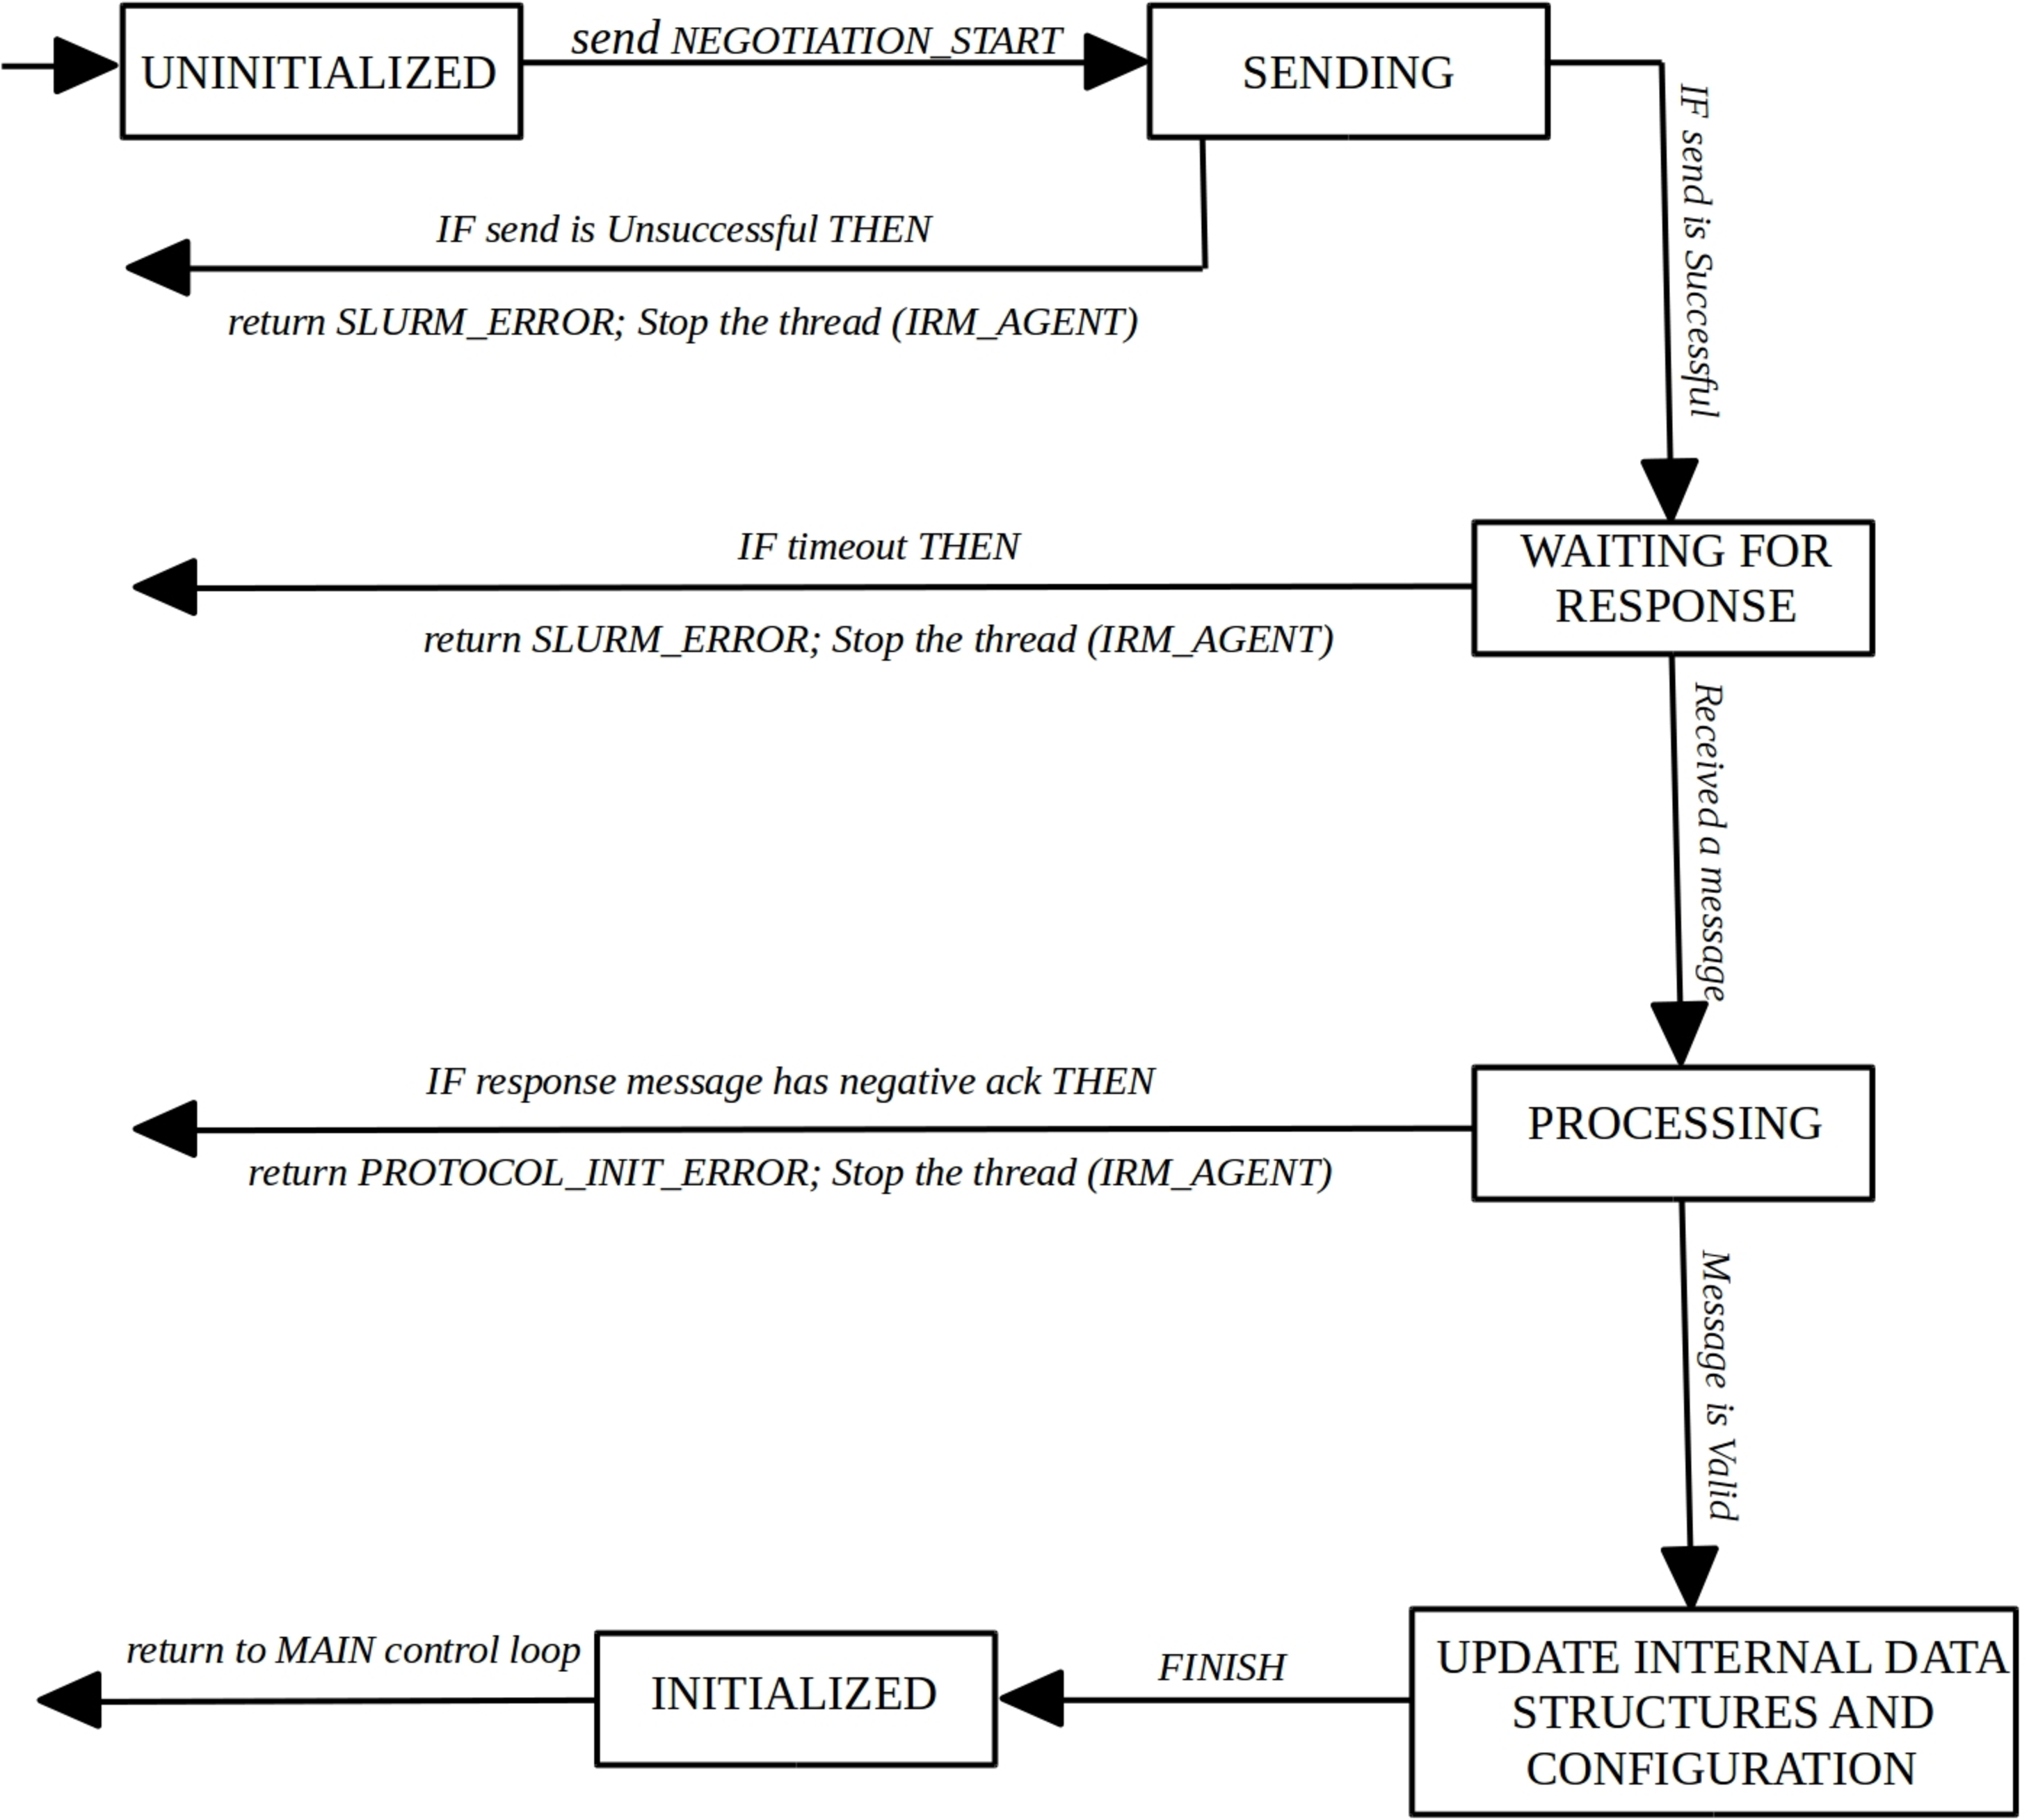
\includegraphics[width=0.9\textwidth, height=90mm]{./figures/Init.pdf}
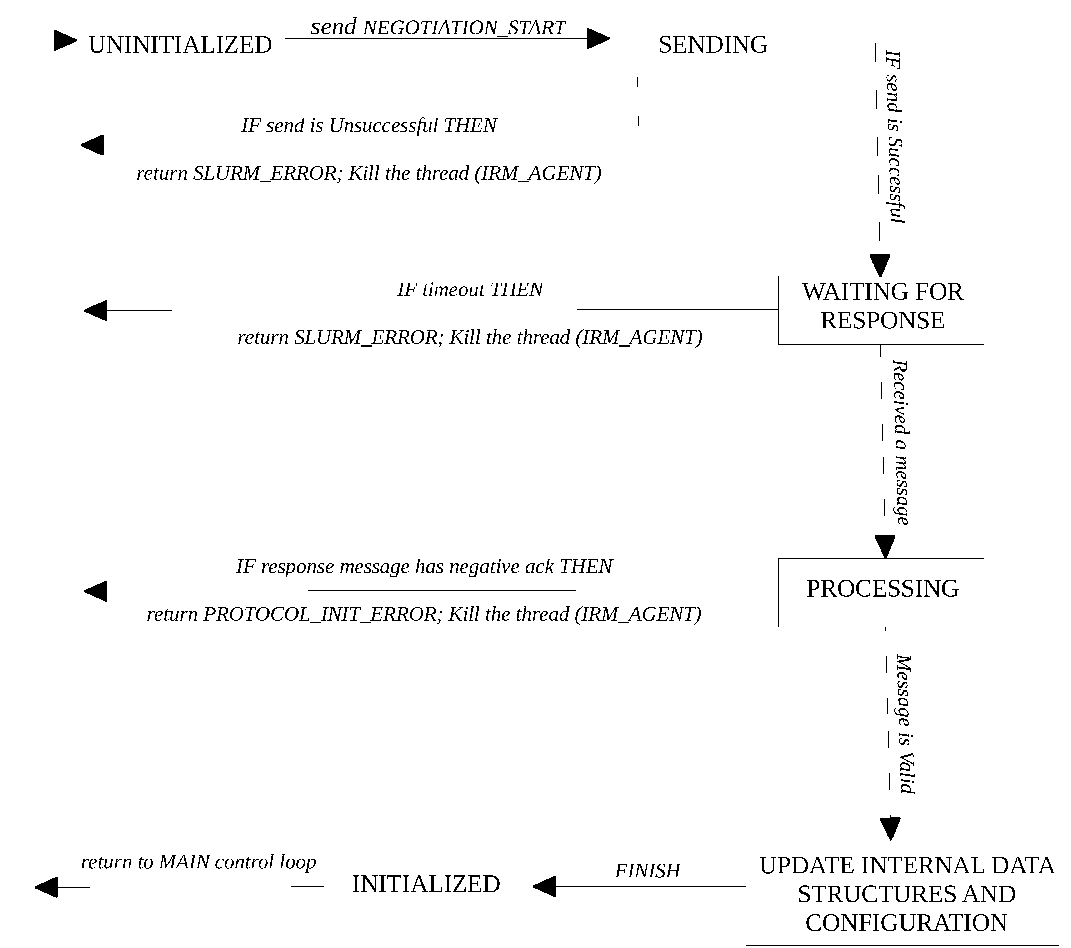
\includegraphics[width=0.9\textwidth, height=90mm]{./figures/Init.eps}
\caption{Protocol Initialization}
\label{fig:Init}
\end{figure}
\vspace{5mm}
\begin{figure}[h]
\centering
%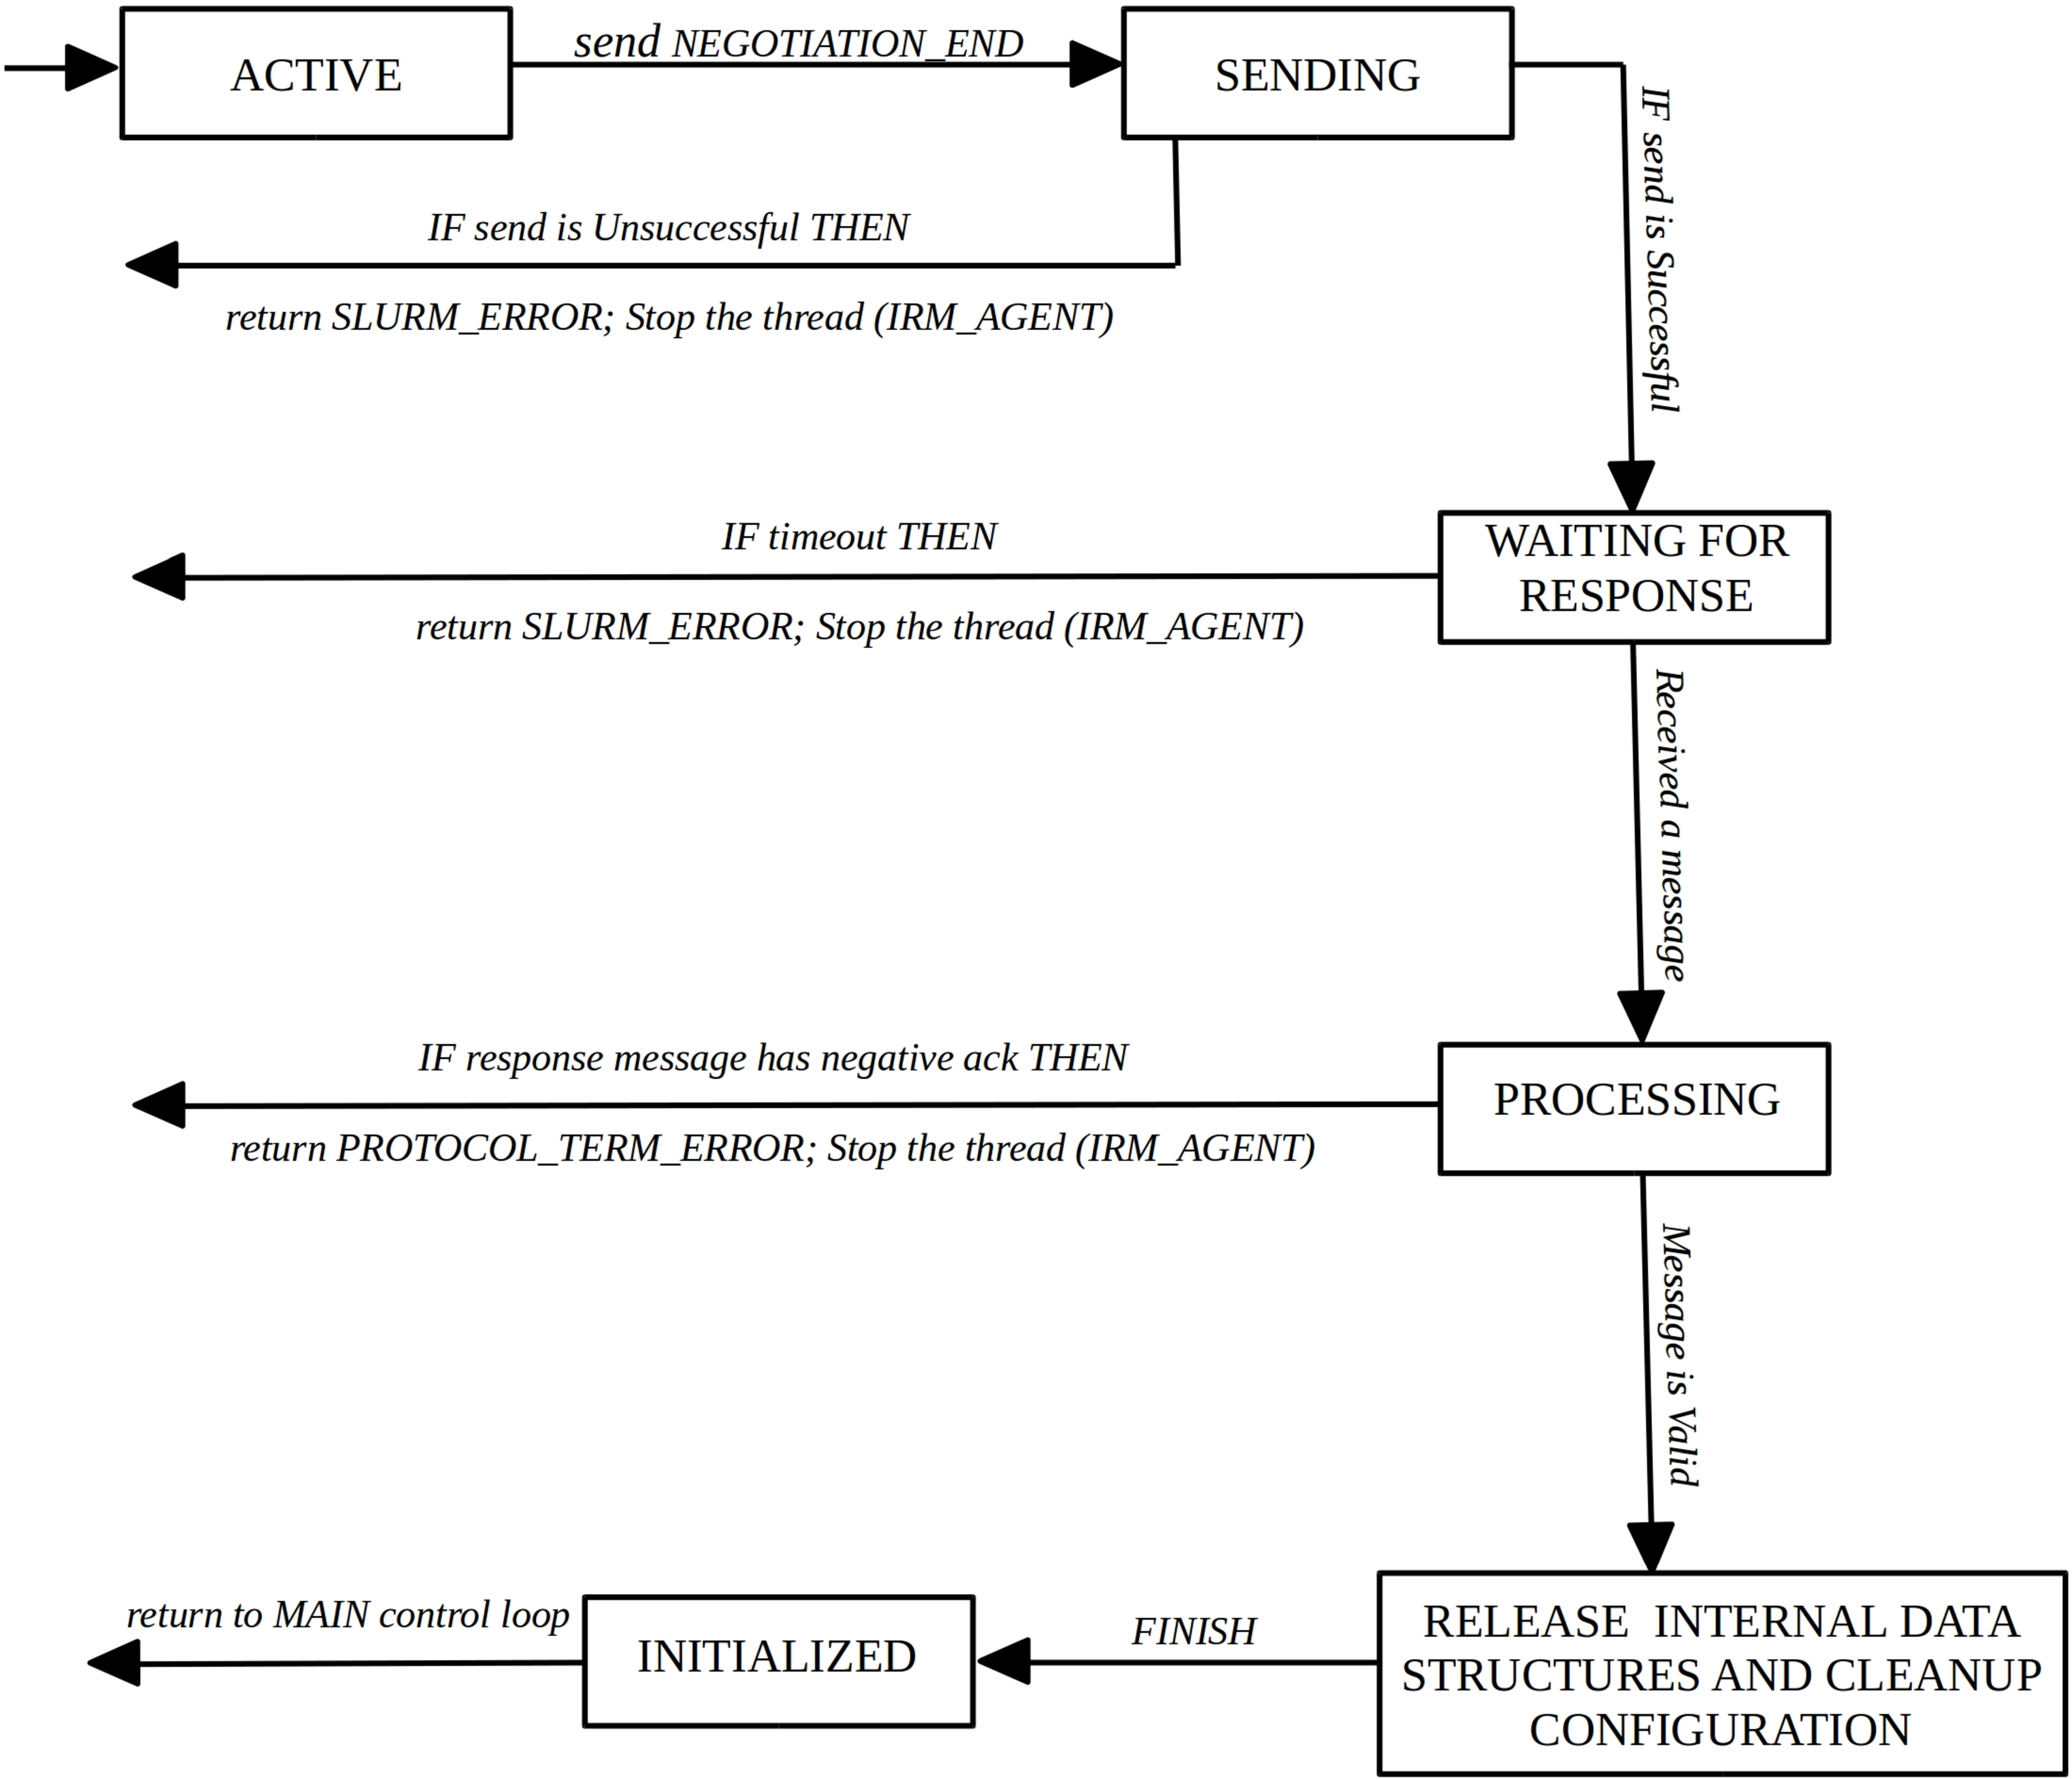
\includegraphics[width=0.9\textwidth, height=90mm]{./figures/Term.pdf}
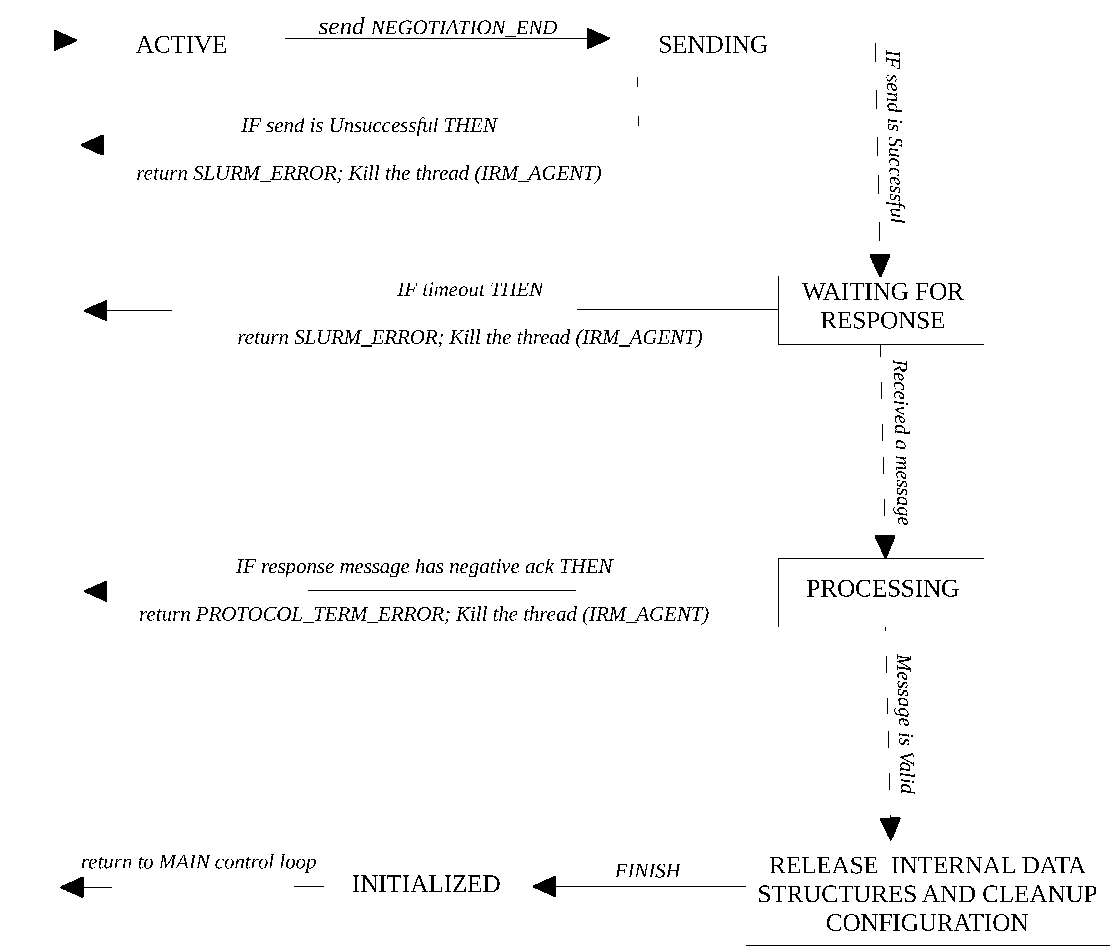
\includegraphics[width=0.9\textwidth, height=90mm]{./figures/Term.eps}
\caption{Protocol Termination}
\label{fig:Term}
\end{figure}
\clearpage
\begin{figure}[h]
\centering
%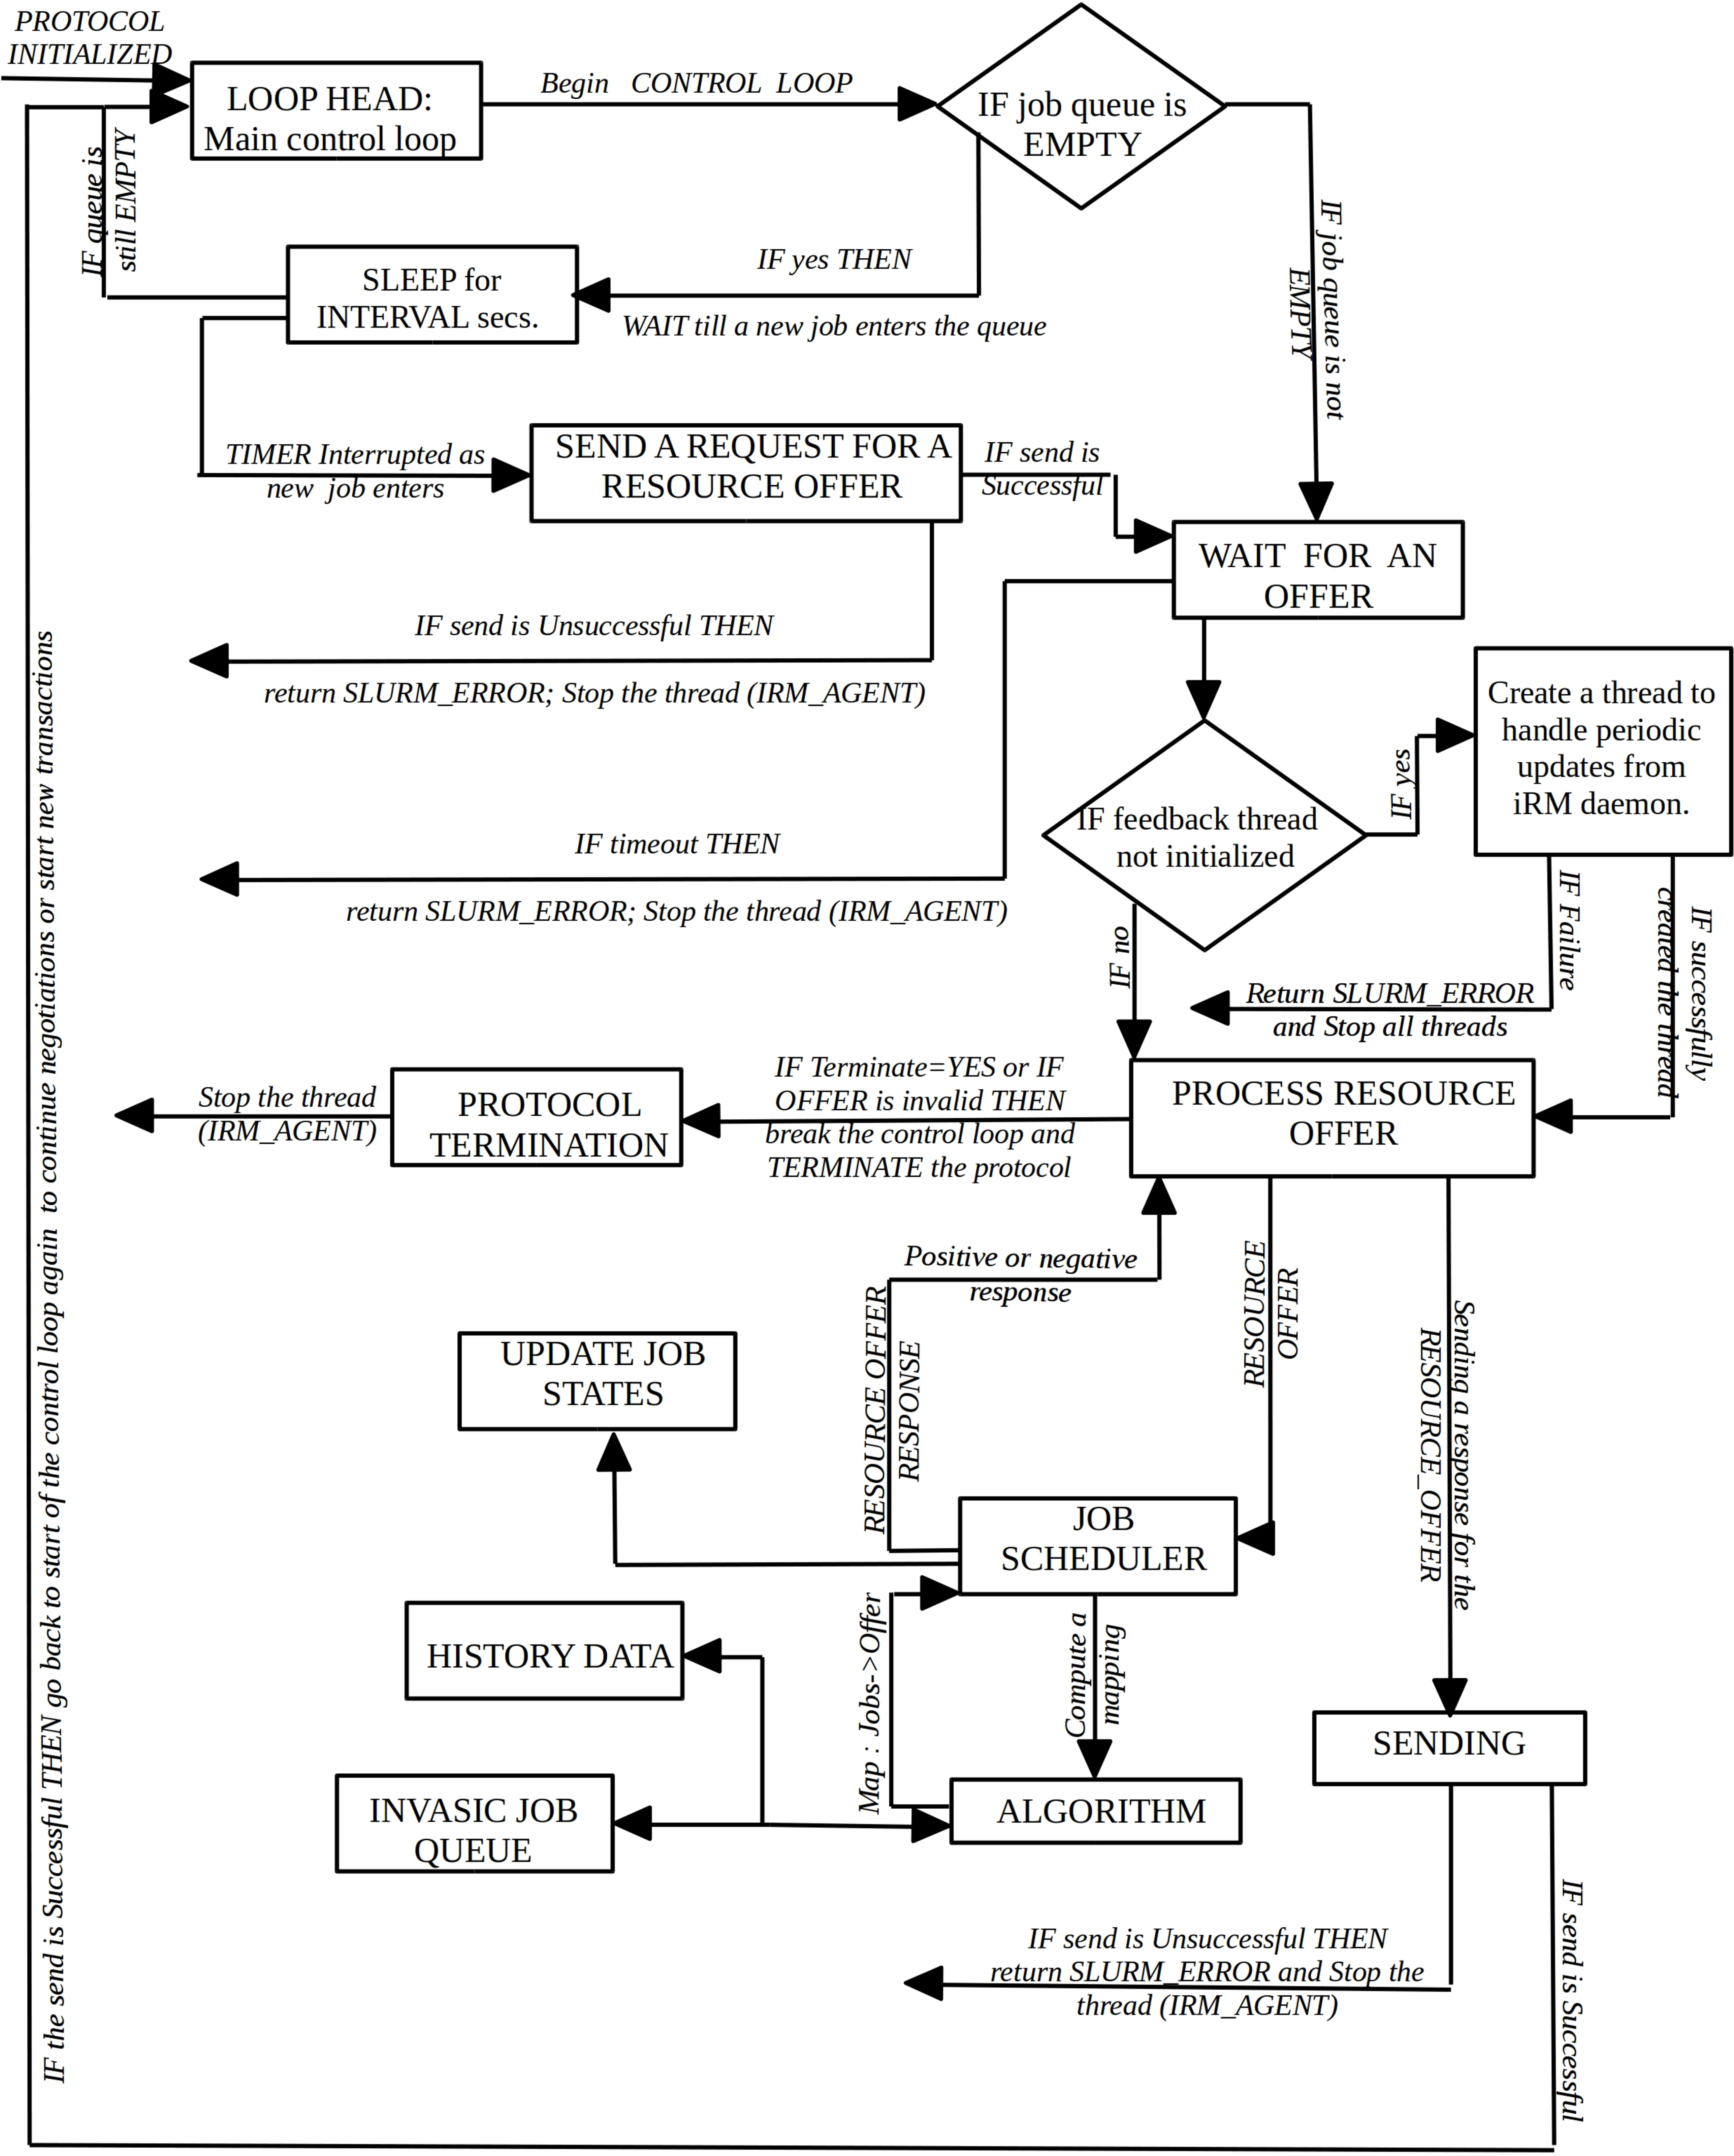
\includegraphics[width=1.0\textwidth, height=210mm]{./figures/Negotiation.pdf}
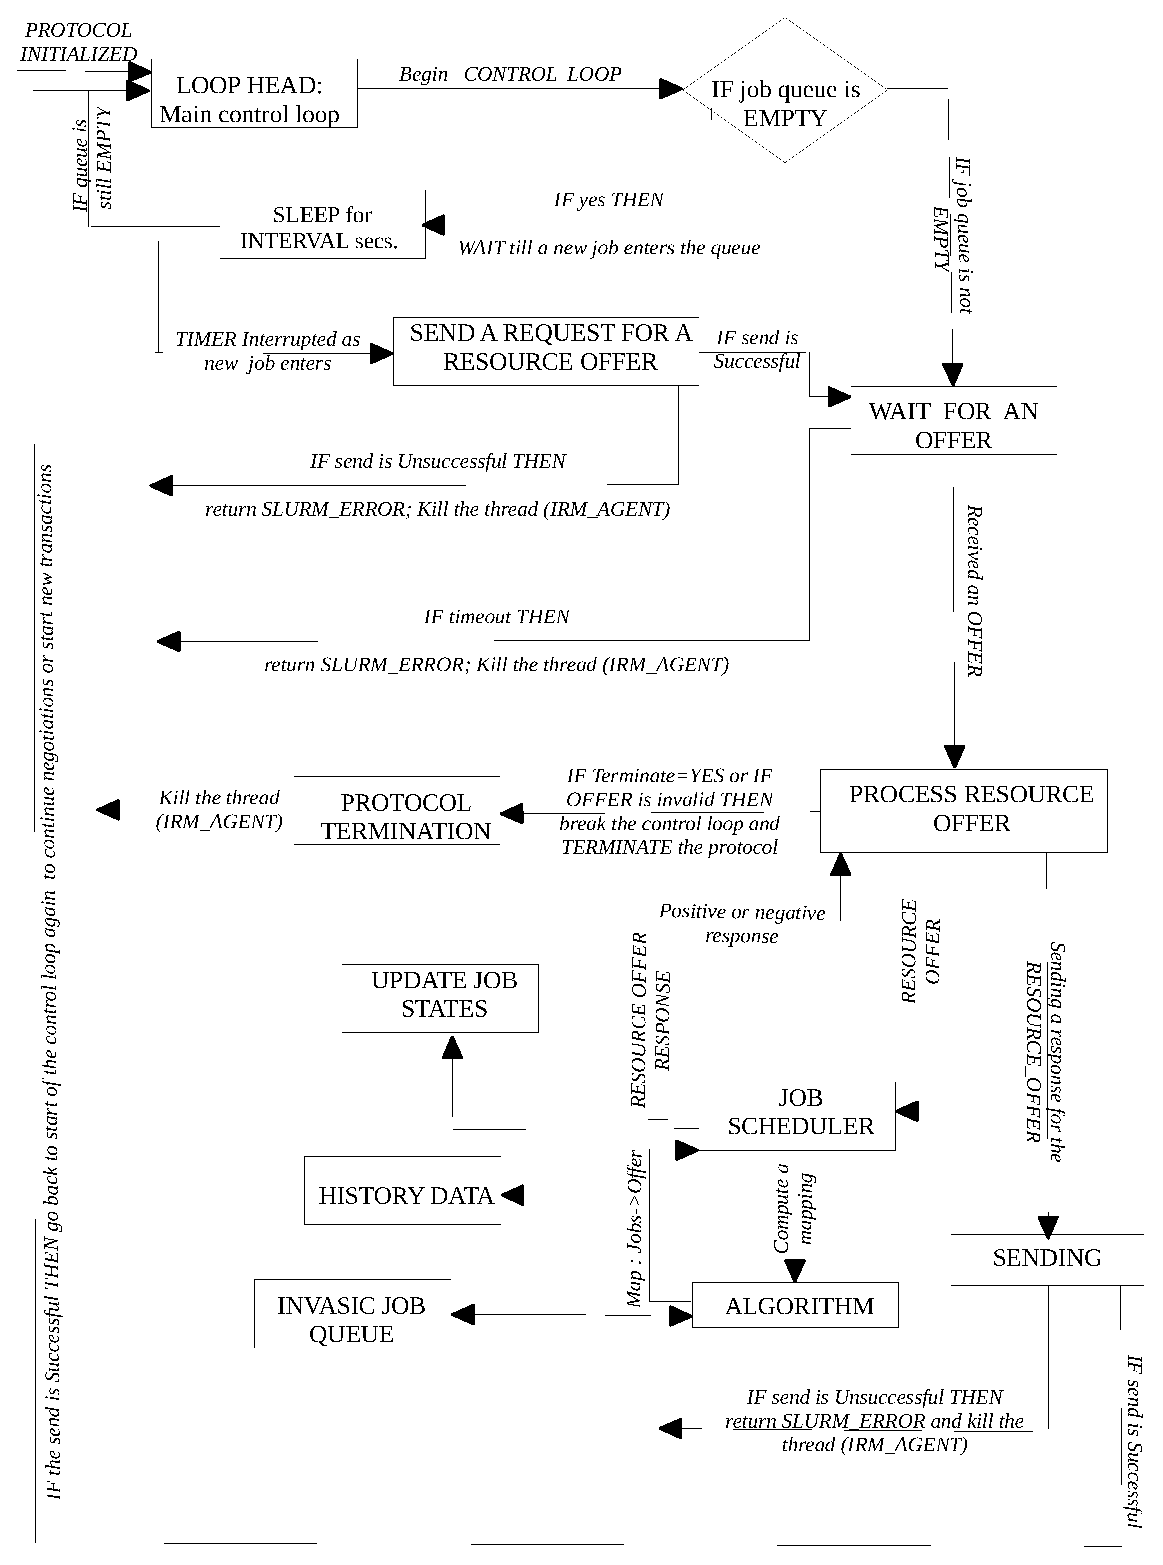
\includegraphics[width=1.0\textwidth, height=210mm]{./figures/Negotiation.eps}
\caption{Negotiation}
\label{fig:Neg}
\end{figure}
\clearpage

\section{Invasive Jobs}
